%!TEX root = ../dokumentation.tex

\chapter{Introduction}

\section{Different kinds of data processing system}

In the modern times of Machine Learning and Big Data analysis the importance of data processing systems increases continuously. More and more systems are being released for Big Data Analysis, for example Spark or Hadoop. Such systems are called \acs{OLAP} - \acl{OLAP}. OLAP has a long history with traditional data warehouse, but with the new world of Big Data they gain even more in importance. Analysis Processing systems are working with groups of data and complex requests. For better analyses it also doesn't only use the current state of a dataset, but also its history. The objective of OLAP systems is to give one unique, consistent view on all data from different sources and extracting information like prediction or other complex information out of these data.\textsuperscript{cmp.\cite{5}}

%https://books.google.com/books?hl=en&lr=&id=eskZA1CFdqMC&oi=fnd&pg=PR9&dq=olap&ots=W4YneSBgRg&sig=VpzggLvlWxFP39aEE1e3FVkErs8#v=onepage&q=prediction&f=false

But still conventional data processing like \acs{ACID} (\acl{ACID}) transactions is needed for regular database requests, for example bank transactions or text messages. Those systems are called \acs{OLTP} (\acl{OLTP}). Those systems are characterized by instant interactions with the business systems with low latency instead of collecting all transactions and process them all at once at one specific time. This was a major step forward in fast data processing in the late 1970s and those systems are still used by almost any company.\textsuperscript{cmp.\cite{6}}

%https://books.google.com/books?id=fV0NAAAAQBAJ&printsec=frontcover&hl=de&source=gbs_ge_summary_r&cad=0#v=onepage&q&f=false

The problem is, that both of these systems need a specific form of their data, so they can't work together on the same dataset. For resolving that problem \acs{HTAP} (\acl{HTAP}) has been created. This enables real-time analytical results, which can help businesses in quick decision making. Therefore are still two copies of the data needed, but with an highly increased synchronization rate between those two data copies.

The Wildfire system, which was developed at IBM Research Lab Almaden, is such an HTAP system. It uses Spark as OLAP engine and an own engine for OLTP. In the following chapters this system and underlying technologies will be presented. Furthermore an experimental study will be described, in which a part of this solution will be deployed on a Cluster system and tested concerning its performance. \textsuperscript{cmp.\cite{7}}

%https://www.informatik-aktuell.de/betrieb/datenbanken/htap-hybrid-transactional-and-analytics-processing.html

\section{Advantage of cluster systems}

Cluster systems are two or more computers connected to each other, so that they can share their resources and can be viewed as one system. Therefore they can be connected physically as well as virtually. Using such a cluster system is typically much more cost-efficient compared to using a single computer, which provides about the same power. But the advantage of such systems doesn't end with a better cost-efficiency.\textsuperscript{cmp.\cite{1}}

%https://www.cc.gatech.edu/~bader/papers/ijhpca.pdf
%CHECK COST EFFICIENCY

First clusters are not only used for one specific purpose, but there are different kinds of cluster configurations, which are build for different objectives.

On the one hand, there are ``Load balancing'' cluster configurations. Load balancing clusters are clusters with the objective to provide better computing performance, like minimizing response time and maximizing throughput.  Therefore it splits the computation in different parts and runs them parallel on different nodes. Through that the capabilities of the systems can be combined.\textsuperscript{cmp.\cite{2}}

%Aho, Alfred V.; Blum, Edward K. (2011). Computer Science: The Hardware, Software and Heart of It.

Furthermore there are ``High availability'' clusters, which are designed to prevent a total break down of the system. For that there are several redundant nodes connected to the system. That means, that when one component fails, a redundant node of this component is used to provide the service. Thereby availability is ensured even if one component fails. The more redundant nodes are used the better will be the availability of a system. To provide an example: If a system has an availability of 90\% it has a downtime of 10\%, which means that the system is not available on 36.53 days per year. If there is a second, redundant and independent node connected to the cluster, which acts as a stand-in for the first system in case of a failure, the downtime of those two systems has to be combined. That means that this cluster would only fail if there is an overlap between the downtimes of those two systems. Resulting of a downtime of 10\% of each system there is a combined downtime of 1\% or 3.65 days per year. If there is a third system connected to the cluster, the downtime will be reduced to 0.1\% or 8.77 hours per year and so on. The job of ``High availability'' clusters is in that to reduce the downtime of the system and to provide a working system almost any time.\textsuperscript{cmp.\cite{3}}

%https://patents.google.com/patent/US6944785B2/en

\begin{figure}[h]
\centering
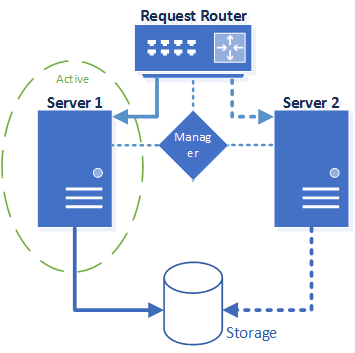
\includegraphics[width=\textwidth/2]{images/ha_cluster_architecture.png}

\textsuperscript{Figure 1.1.1 ``High availability'' cluster architecture}
\end{figure}

Figure 1.1 shows an example architecture of such a ``High availability'' cluster. There are two servers, whereby one server is a replication of the other one. The request router handles the incoming requests and leads them to the active server. If there is a system failure of the active server, the manager will recognize that, and sends a message to the request router to change the request address to the other server. From now on this server will deal with all the requests. Also there is a shared storage for both of the servers in one database. No matter which one is active they can both access this database.\textsuperscript{cmp.\cite{4}}

%https://confluence.atlassian.com/bitbucketserver/high-availability-for-bitbucket-server-776640137.html

But those advantages don't have to stand alone, but they can also be combined, so that you can provide high availability as well as high performance. Because there is an continuously increasing amount of calculations to be made cluster systems are becoming more and more important in modern IT for providing a solution for both problems.

\section{Introduction to IBM Research Cloud}

For a few years there has been a trend to move from local, physical devices to centralized Cloud platforms. This has different advantages like dynamically allocation of computing power and more cost-efficiency. The reason for this is because often there are unused resources on physical devices, because most systems don't need all of their power all the time. Through outsourcing this computing power to the Cloud the resources are only used where they are needed. This increases the cost effectiveness eminently, because not every physical device needs backup resources for situations, in which more computing power is needed. Instead with the cloud it is possible to request more resources when needed and to release them when they are not needed any longer.\textsuperscript{cmp.\cite{8}}

%https://www.skyhighnetworks.com/cloud-security-blog/11-advantages-of-cloud-computing-and-how-your-business-can-benefit-from-them/

In Research there is often a lot computing power necessary for testing, calculating and building projects and experiments. Therefore every lab has several own physical devices. But currently there is also a trend in Research projects to move to Cloud devices for sharing resources and save costs. That is the reason why IBM started its ``IBM Research Cloud'', hosted on \acs{iRIS} (\acl{iRIS}) \acs{IMS} (\acl{IMS}). This is a self-service platform, which provides Cloud based solutions for IBM Researcher on request for specific resources.\textsuperscript{cmp.\cite{9}}

%internal sources

IBM Research Cloud itself provides virtual devices as well as virtual \acs{GPU} (\acl{GPU}) devices. Virtual devices mimics physical hardware but without the need of an isolated physical machine. Instead its just splitting some computing power of a big cluster via Software and makes the system believe, that it would be an isolated hardware device. Virtual GPU devices are differentiated by an additional Graphical Unit, which provides the virtual device even more computing power and relieves the \acs{CPU} (\acl{CPU}) in some tasks.\textsuperscript{cmp.\cite{10}, \cite{11}}

%https://www.techopedia.com/definition/12632/virtual-device (?)
%https://www.nvidia.com/en-us/design-visualization/solutions/virtualization/ (?)

Besides the creation and deletion of virtual devices, the Research Cloud also provides operations like hard/soft reset or rebooting a device. Additionally it also provides the opportunity to create an image of an existing virtual device and creating a new one from this image. Through that you can keep your configurations and files from your old device and create a device based on those configurations without the need of installing everything up from the beginning.

In the following report this Research Cloud will be used to setup a Kubernetes Cluster with several virtual devices and try to run Wildfire using this Cluster.

\section{Project objective}

The objective of this project was split in two parts: First to experiment with the Wildfire post-groomer on a Kubernetes cluster to figure out how to setup a Kubernets cluster and how Spark in general or a specific Wildfire version can be run on it. It also includes making some performance tests on those and evaluate corresponding results. 

The second objective was to evaluate the Research Cloud as possible replacement for physical devices in the future. This was motivated because of the initiative to move back from a high amount of physical devices for each lab to shared, virtual devices on the Cloud. Thereby first the workflow for creating and deleting devices on the Cloud, manually as well as automated via an \acs{API} (\acl{API}), should be figured out and then some performance comparisons to physical devices should be made.

Last those steps should be combined in a software for automated testing the Wildfire postgroomer within a Kubernetes cluster running on Cloud devices. This should enable easier and faster testing in the future and a better view on the overall performance of the Cloud devices and Wildfire within a Kubernetes cluster.
